\section[Usage]{Usage - its not just me that thinks it is good}
\label{variantcalling-sec:usage}
As amazing as published open source software is, its real value is in the re-usability and portability. Many published software packages are not maintained or not even functional even though they are published. While I developed these joint somatic variant calling workflows to deal with a challenge I faced, many other people even just at the same institute have already shown interest and some research groups are already using the software to analyse their multi-sample data.

\begin{figure}[!ht]
\centering
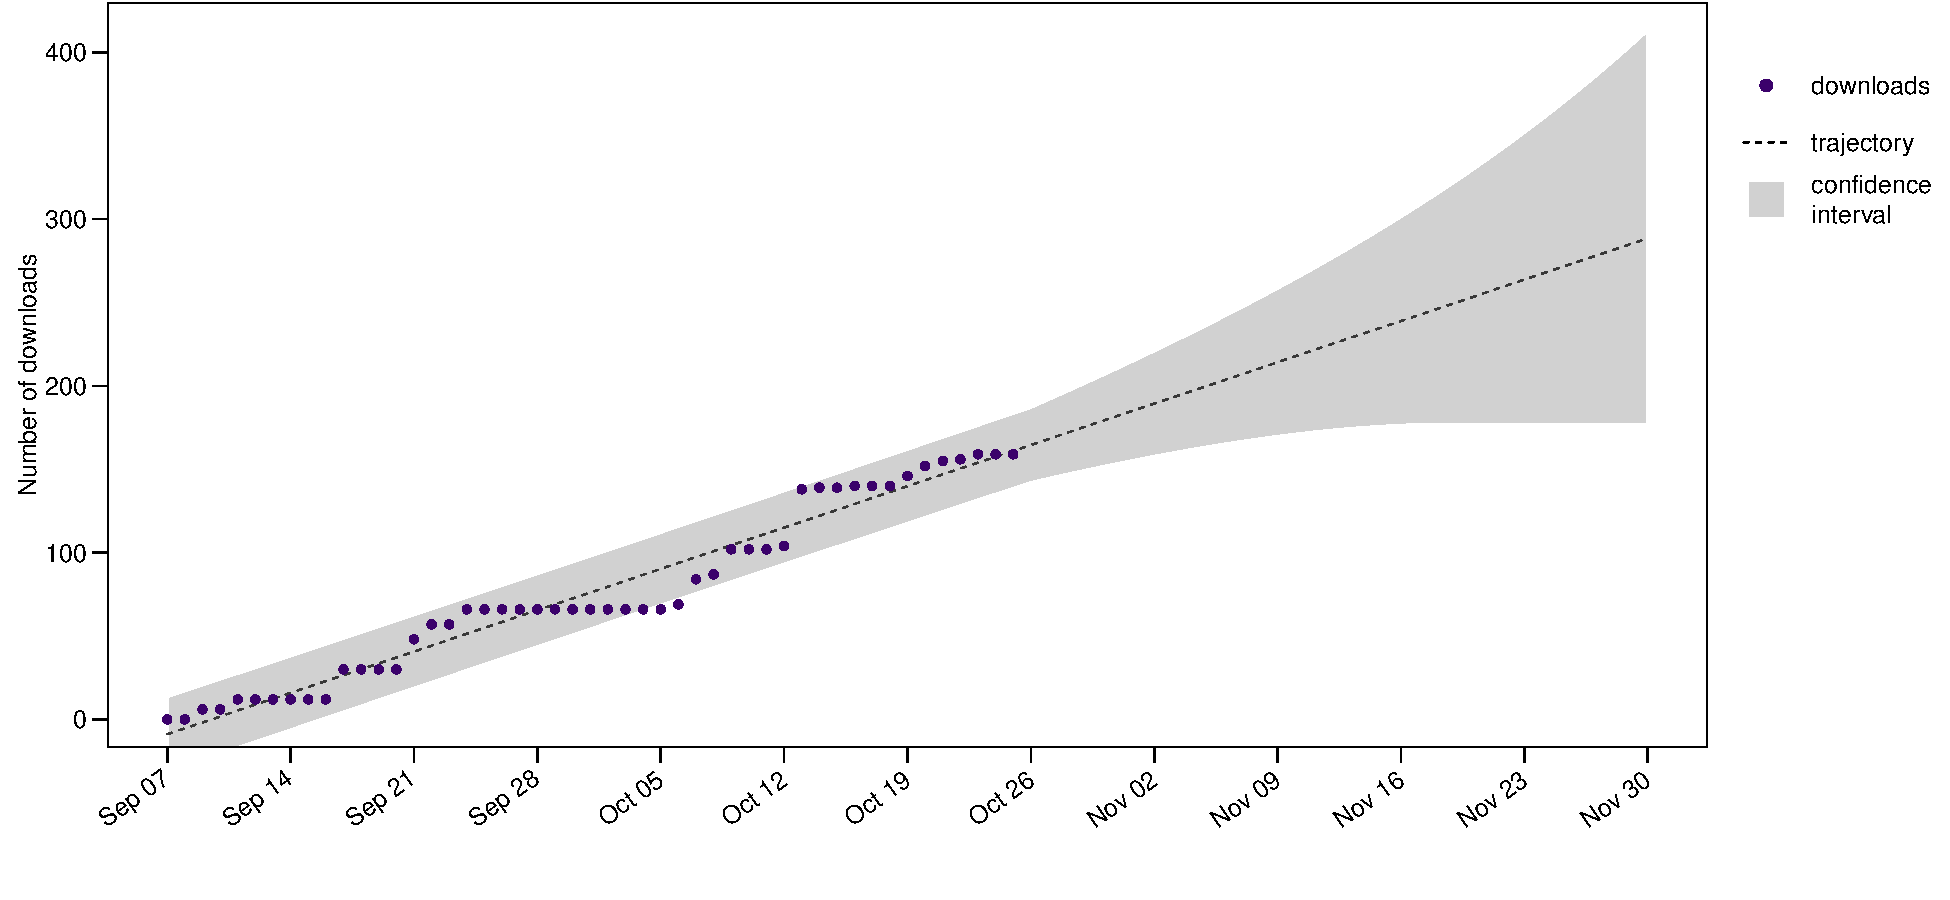
\includegraphics[width=.99\linewidth]{Figures/dawsontoolkitDownloads.pdf}
\caption[Usage statistics joint workflows]{Cumulative download numbers of the ``dawsontoolkit`` docker container since publication of the manuscript; Actual counts are shown as dots, with smoothed trajectory depicted as dotted line with the 95\% confidence interval shown as a grey background; confidence interval has been adjusted with exponential decay of prediction accuracy with distance from the last data point; Start date 7$^{th}$ September 2021 (publication of method); End point prediction 8$^{th}$ April 2022 (End of candidature)}\label{fig:usageStats}
\end{figure}

To have some proxy of the usage statistics of the workflows, I recorded the download numbers of the ``dawsontoolkit`` docker container after the publication of the manuscript. The cointeriner only consists of software for refiltering and joint analysis of the workflows . Obviously, this is an imperfect measurement, as people can reuse a downloaded container as often as they want, which would not appear in the count and similarly, just because the container was downloaded, the analysis might not have been used. However it still shows  an interaction and an interest in the methods. The download numbers show a sustained stable increase in downloads (\autoref{fig:usageStats}). This suggests, that there is a need in the methods, rather than a simple curiosity after publication, which hopefully will facilitate a higher quality analysis of future projects and therefore lead to a better understanding of cancer evolution and heterogeneity.
